\chapter{Methodology}

% TODO reference why this is being referred to as agile via the agile manifesto
% TODO reference gannt chart in PID in appendix
At the start of the project a high level representation of the research and development steps required to complete the project was created. Theses steps were allocated a time frame and a sprint was planned at the start of each time frame.

While each sprint was different, sprints broadly involved defining a clear goal and pursuing it until the end of the sprint window. While the sprint windows were not strict cut offs, the primary focus of my time would change upon the start of a new sprint window.

% TODO bottom two paragraphs can come at the top
This workflow is best described as a modified agile scrum methodology with a variable and flexible sprint window for each objective.

This chapter will chronologically outline the steps planned and taken in the progression of the project.

% TODO reference this to PID use agile to explain why headings / steps changed

% TODO as well as chapter intro include chapter conclusion
\section{Steps Taken}

\subsection{Research Potential Projects}

The first step in this project was to identify potential project ideas. This was done with brainstorming, both by thinking about the project and talking about it with others.

The project ideas broadly fell into two categories, engineering, where the objective is to produce an application, and research, where the objective is to provide insight or an answer to an unknown.

A personal goal for me in this project was to develop my skills in machine learning and artificial intelligence. Evaluating the iArsenic models and producing alternative models with machine learning appealed to me as the most exciting option. Additionally, because the project already contained hours of existing work, the objectives of the project could build off this work instead of starting from scratch. This enabled higher level and higher impact objectives to be set. 

As Dr Mohammed Hoque agreed to be the client to this project I was able to commit to this project, confident in knowing it had purpose and direction from the client.

\subsection{Clarify the Project Objectives}

Originally the vision of the project was to develop machine learning based models and compare their performance to the existing iArsenic models.

This initial vision is however does not define several key aspects of the project. How does one evaluate the performance of an iArsenic model? How does this compare to an evaluation of a machine learning based model? What is the purpose of developing new models and comparing them to the existing ones?

Ultimately the desired outcomes were clearly defined as follows:

% TODO desired outcomes could probably live somewhere else
\textbf{Desired Outcomes}

\begin{enumerate}
  \label{desired_outcomes}
  \item To evaluate the existing models
  \item To compare the performance of the existing models with typical machine-learning-based models
\end{enumerate}

Desired Outcome 1 was requested from the client. Evaluating the models informs the client of how each iteration of the models have impacted their performance and, because this model is deployed, verifies the quality of the predictions being made in deplyoment.  While the existing models were developed with expert knowledge, prior to the evaluations conducted in this project, the performance of the models was unknown.

The purpose of desired outcome 2 comes from \cite{Fleming2021}'s assertion that machine learning should be part of Earth and Environmental Science (EES). iArsenic provides an opportunity for a case study where expert system models can be compared to supervised learning models. 

It is difficult to ascertain what level of sophistication of machine learning models an EES graduate would reasonably be able to implement.  Because supervised learning algorithms are standardised in scikit-learn, this project suggests that these models are the kind that an EES graduate with approximately 2 undergraduate modules of machine learning could implement.

\subsection{Research Applied Machine Learning Methodologies}

To design implement and evaluate machine learning models for iArsenic, I first had to research machine learning to understand what specific areas in machine learning could be applied to this dataset to achieve the desired outcomes of the project and then had to develop these models in code to gain the practical experience required.

Chapter 2 of \cite{Aurélien2017}'s book Hands-On Machine Learning with Scikit-Learn and TensorFlow was the primary resource for breaking through the barrier of theoretical knowledge, gained from written sources such as \cite{Caruana2006} which compares several supervised machine learning models in different applications, to actually producing my own implementations of these models.

% TODO, could all the code in this section be moved to experiment design
\subsection{Understanding the iArsenic Codebase}

The iArsenic codebase provided the following key functions:

\begin{enumerate}
  \label{ia_functions}
  \item Producing a standard dataset
  \item Generating iArsenic models from a dataset
  \item Generating predictions from these generated models
\end{enumerate}

By looking at the iArsenic website and know it produced a model based on existing data which could produce a prediction for a given data point, it was clear that the project included this functionality.

To learn how to achieve this functionality, I would read the iArsenic code in GitHub and experiment with it as an npm package.

\textbf{Producing a standard dataset}

The iArsenic script csv-to-json.js makes exporting a standardised dataset trivial.

This function is implemented in the project via an package script:

\begin{figure}[h]
\begin{minted}[linenos, breaklines]{json}
"scripts": {
    "load-src-data": "mkdir well_data ; node node_modules/preprocessing/preprocessing/cli/csv-to-json.js -p node_modules/preprocessing/data/*.csv -o well_data/src_data.json",
\end{minted}
\label{fig:x load_ia_data}
\caption{package.json snippet showing script to load data from iArsenic}
\end{figure}

See the file at \url{https://github.com/portsoc/iArsenic/blob/master/preprocessing/cli/csv-to-json.js}

\textbf{Generating iArsenic models from a dataset}

To verify that a model can generalise to new cases, it must be trained on a subset of the data and tested on a separate subset of data which it has not been previously exposed to. In the iArsenic webapp, the models are trained on the entire source dataset. See \ref{fig:x imp_iam_webapp} on page \pageref{fig:x imp_iam_webapp} for an flowchart showing this implementation.

Generating the models on a training subset of the data was done by passing 4 of the 5 subsets of the data, after the data was split into 5 for k-folds cross validation, to the iArsenic model generator. This was done for each of the 5 subsets of the data for each of the 3 iArsenic models. See \ref{fig:x programmatically_gen_ia_model} on \pageref{fig:x programmatically_gen_ia_model} to see the code that achieved this.

\begin{figure}[h]
    \centering
    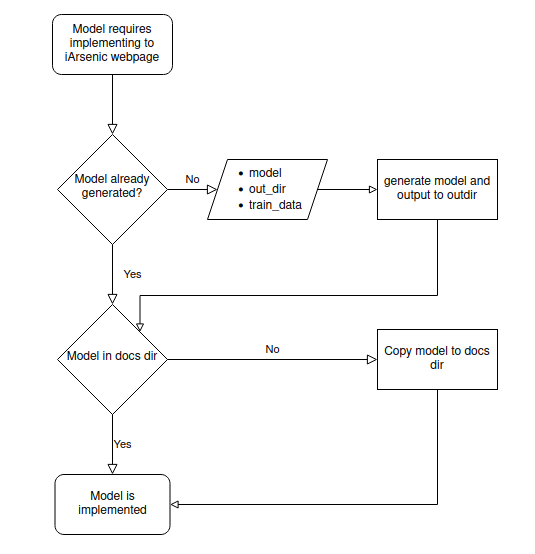
\includegraphics[scale=0.6]{figures/implement_ia_model_to_webapp.png} 
    \caption{Flowchart showing process to implement model in iArsenic webapp}
    \label{fig:x imp_iam_webapp}
    \small The code that generates the models can be found at: \url{https://github.com/portsoc/iArsenic/blob/master/preprocessing/cli/produce-aggregate-data-files.js}
\end{figure}

\begin{figure}[h]
    \begin{minted}[linenos, breaklines]{python3}
def gen_model(train_src, out_dir, model):
  if not os.path.exists(out_dir):
    os.mkdir(os.path.join(out_dir))

  cmd = [
    'node',
    'node_modules/preprocessing/preprocessing/ cli/produce-aggregate-data-files.js', 
    '-m',
    model,
    '-o',
    out_dir,
    '-p',
    train_src,
    'node_modules/preprocessing/data/mouza-names.csv',
  ]
  stdout = check_output(cmd).
    decode(sys.stdout.encoding).
    replace('\n', '')
    
  print(stdout)
      \end{minted}
    \caption{Python code used to programmatically generate iArsenic models}
    \label{fig:x programmatically_gen_ia_model}
\end{figure}

\textbf{Generating predictions from generated iArsenic models}

The web application index.html file shows a script.js file is used, in this file a global function called produceEstimate is called from the estimator.js script. See \ref{fig:x produce_estimate_call} on \pageref{fig:x produce_estimate_call} to see this function call.

Comments in the estimator.js file indicate that this file is a component of the generated model. Therefore this function is used as a generic entry point for producing estimates for each model. Because model5 requires a parameter containing Mouza regional data to be but model3 and model4 do not, the implementation of this function call depends on the model being used. See \ref{fig:x programatically_gen_ia_predictions} page \pageref{fig:x programatically_gen_ia_predictions} to see this dual implementation.

\begin{figure}
    \begin{minted}[linenos, breaklines]{python3}
    const estimate = produceEstimate(aggregateData, inputs.division, inputs.district,
      inputs.upazila, inputs.union, inputs.mouza, inputs.depth, inputs.colour, inputs.utensil, inputs.flooding);
    \end{minted}
    \caption{Code used in iArsenic to produce estimate from a model in the webapp}
    \label{fig:x produce_estimate_call}
    \small The file containing this code can be found at: \url{https://github.com/portsoc/iArsenic/blob/master/docs/script.js#L340-L341}
\end{figure}

\subsection{Developing New Models}

To familiarise myself with implementing machine learning models, I initially followed the tutorial in Chapter 2 of \cite{Aurélien2017}'s book Hands-On Machine Learning with Scikit-Learn. I then implemented 4 separate supervised learning models on 25 datasets.

\begin{landscape}
    \begin{figure}[h]
        \centering
        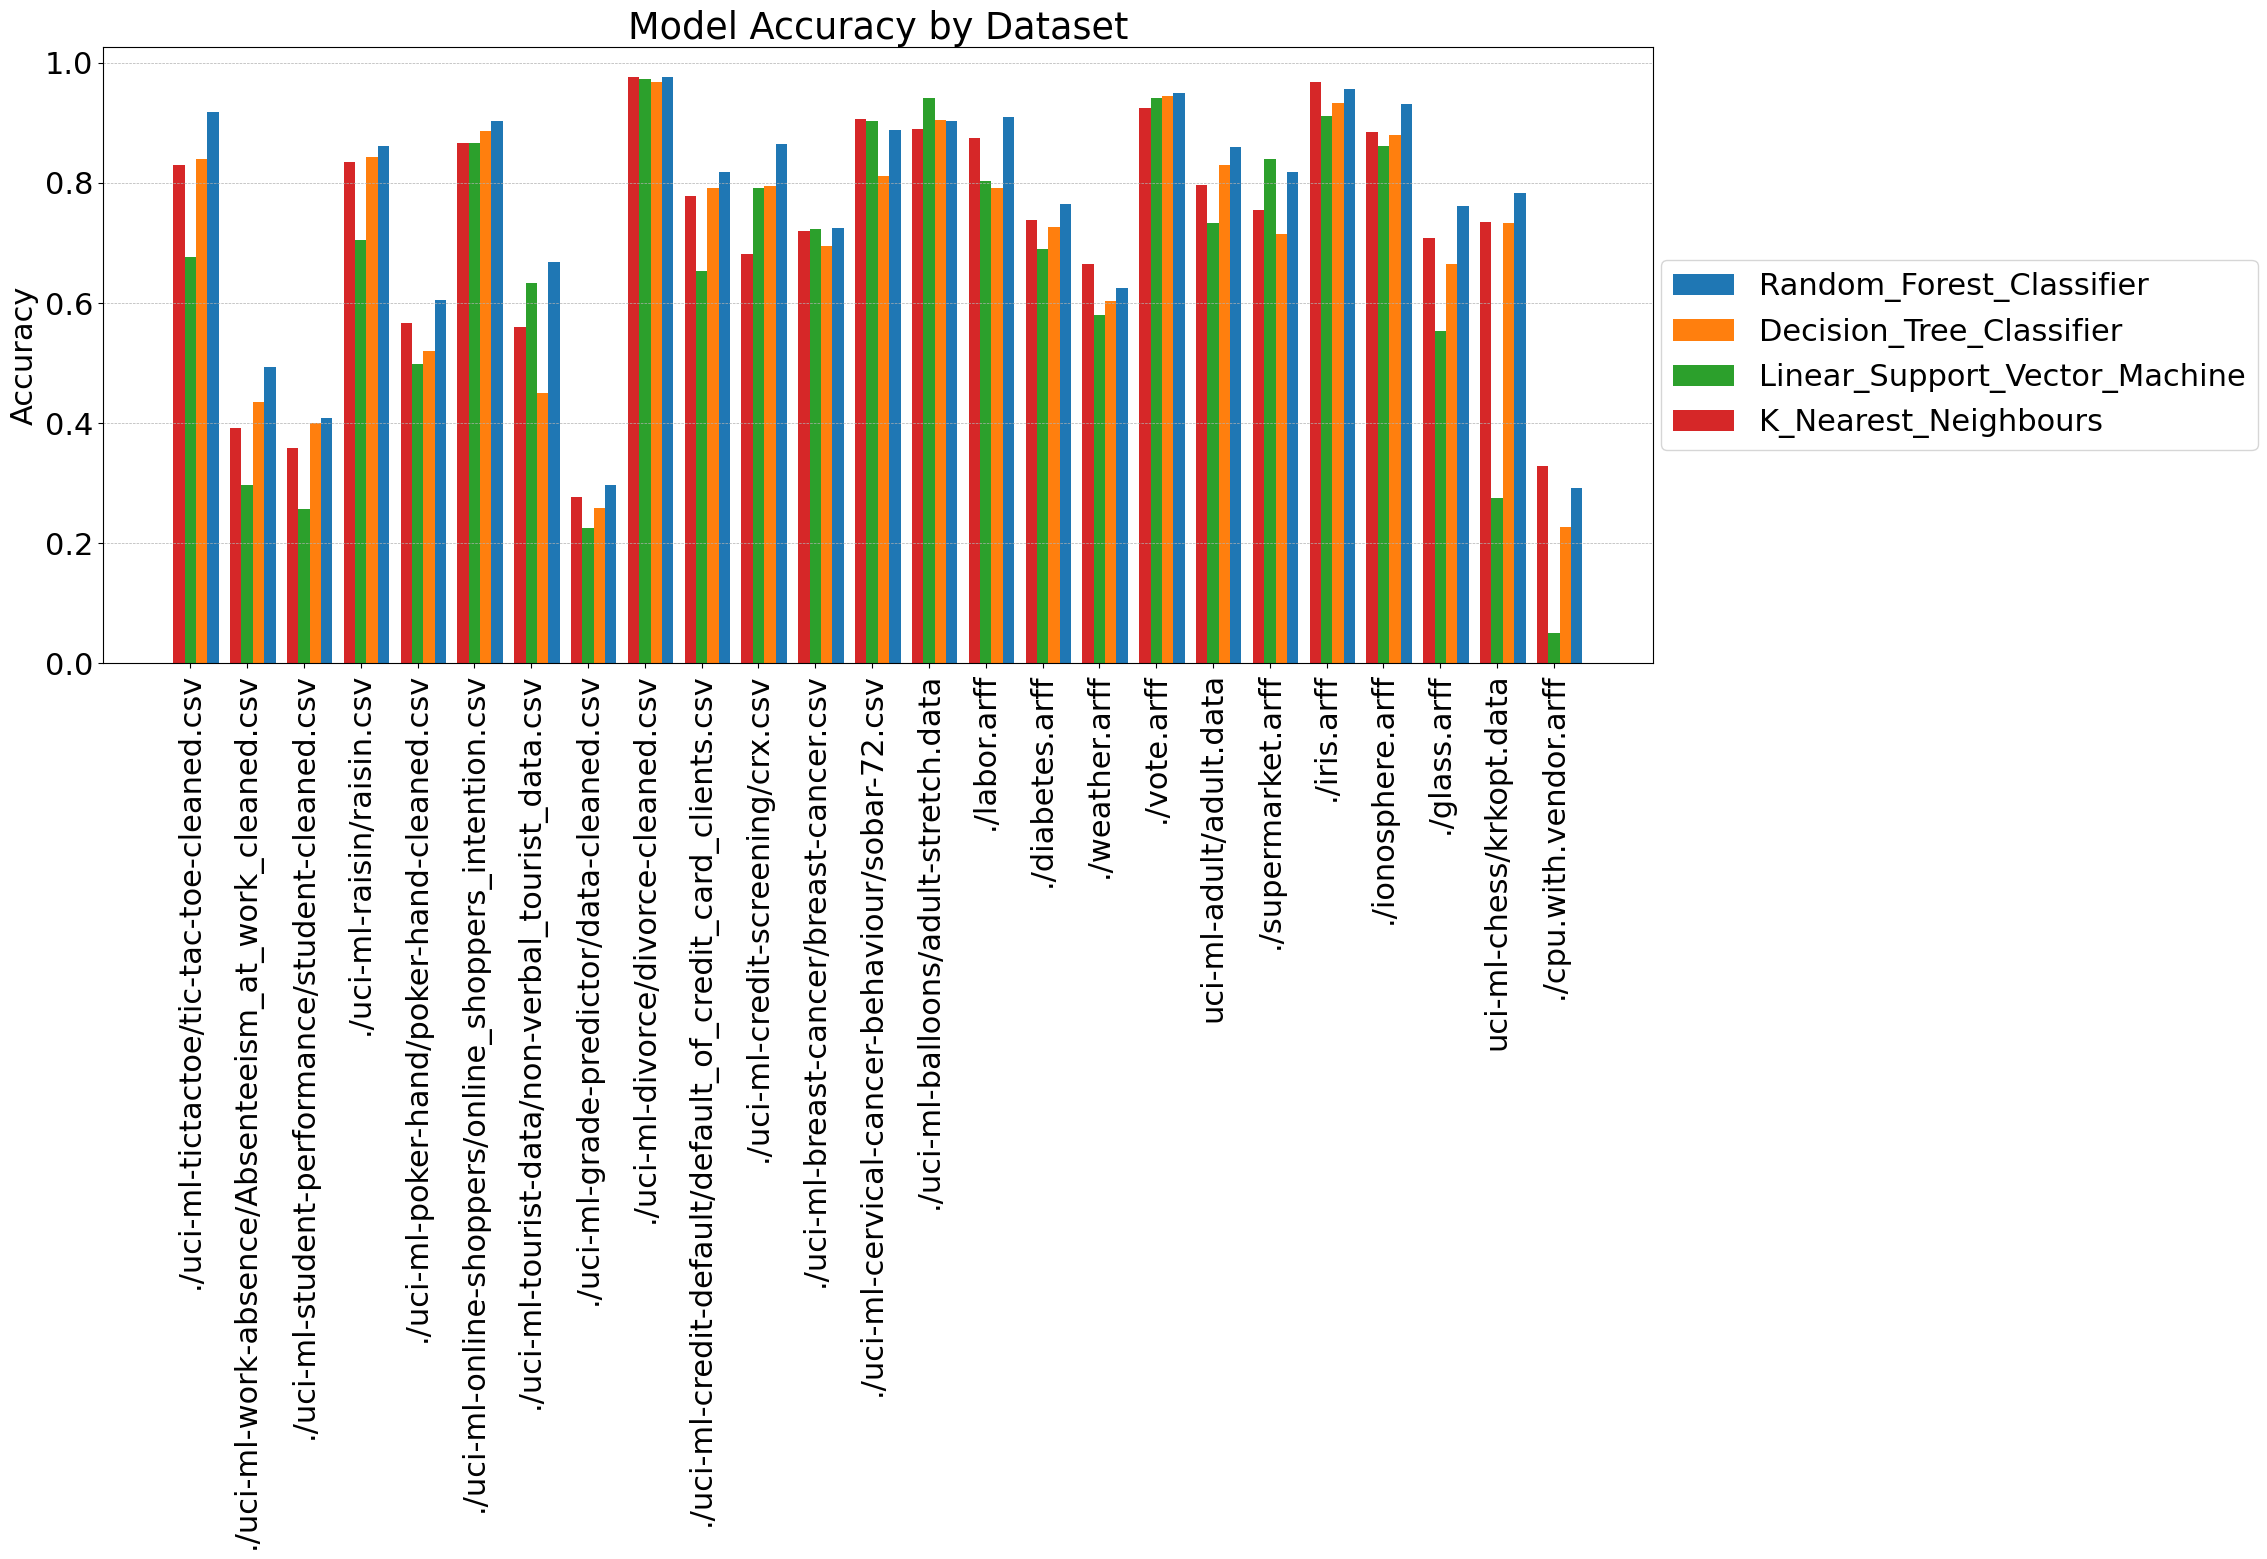
\includegraphics[scale=0.375]{figures/4_models_25_datasets.png} 
        \caption{Summary of results of supervised model implementation practice}
        \label{fig:x 4_m_25_d}
    \end{figure}
\end{landscape}

\subsection{Integrating iArsenic and scikit-learn}

The prototype implementations of both iArsenic and machine learning based models allowed each model to take input data and produce estimations individually. 

Because it takes multiple days to run every experiment required, it is not practical to have a human run each model individually, as the time taken between an experiment finishing and the next starting will depend on when the person gets around to it. By making the models run programmatically this is not an issue. It also allows the project to be more portable, allowing it to be run on a remote server or high performance computer.

To run both NodeJS based iArsenic models and Python based scikit-learn models an integration layer between Python and NodeJS had to be created. Python was chosen as the main program to run the NodeJS code from as a personal preference. Using NodeJS would also have been a reasonable choice.

The iArsenic models are run from Python by passing data over the storage drive as CSV files. See function gen\_ia\_predictions in \ref{fig:x py_call_node} which calls the script containing the code snippet in figure \ref{fig:x programatically_gen_ia_predictions}, passing a filepath to a CSV file of datapoints and reading the CSV returned from the NodeJS script which generated a CSV file containing predictions for the datapoints passed, for a specified iArsenic model.

\begin{figure}[h]
    \begin{minted}[linenos, breaklines]{Python}
def gen_ia_predictions(test_src, stain_color, model, k_fold):
  cmd_arr = [
    'node',
    './models/model_utils/iarsenic-wrapper.js',
    test_src,
    stain_color,
    model,
    str(k_fold),
  ]

  stdout = check_output(cmd_arr).decode(sys.stdout.encoding).replace('\n', '')
  df = pd.read_csv(stdout)
  
  df['Prediction'].replace('highlyPolluted', 'polluted', inplace=True)
  df['Prediction'].replace('We do not have enough data to make an estimate for your well', 'polluted', inplace=True)

  return df['Prediction']
        \end{minted}
    \caption{Python script used to call NodeJS script which produces predictions for an iArsenic model}
    \label{fig:x py_call_node}
\end{figure}

\begin{figure}[h]
    \begin{minted}[linenos]{javascript}
  const estimate = (() => {
    if (model === 'model5') {
      return produceEstimate(
        divisions,
        div,
        dis,
        upa,
        uni,
        mou,
        depth,
        colour,
        utensil,
        flood
      );
    } else {
      return produceEstimate(
        divisions,
        div,
        dis,
        upa,
        uni,
        depth,
        colour,
        utensil
      );
    }
  })()
      \end{minted}
    \caption{NodeJS code which will generate a prediction for a datapoint from a passed CSV file. This code is run for each row of the CSV file.}
    \label{fig:x programatically_gen_ia_predictions}
\end{figure}


